% Gemini theme
% https://github.com/anishathalye/gemini

\documentclass[final]{beamer}

% ====================
% Packages
% ====================

\usepackage[T1]{fontenc}
\usepackage{lmodern}
\usepackage[size=custom,width=120,height=72,scale=1.0]{beamerposter}
\usetheme{gemini}
\usecolortheme{pnnl}
\usepackage{graphicx}
\usepackage{booktabs}
\usepackage{tikz}
\usepackage{pgfplots}
\pgfplotsset{compat=1.14}
\usepackage{anyfontsize}
\graphicspath{{img}}

% ====================
% Lengths
% ====================

% If you have N columns, choose \sepwidth and \colwidth such that
% (N+1)*\sepwidth + N*\colwidth = \paperwidth
\newlength{\sepwidth}
\newlength{\colwidth}
\setlength{\sepwidth}{0.025\paperwidth}
\setlength{\colwidth}{0.3\paperwidth}

\newcommand{\separatorcolumn}{\begin{column}{\sepwidth}\end{column}}

% ====================
% Title
% ====================

\title{Minibatching Offers Improved Performance for Second Order Optimizers}

\author{Eric Silk \inst{1} \and Swarnita Chakraborty \inst{2} \and Dasgupta Nairanjana \inst{2} \and Andrew Lumsdaine \inst{3} \and Tony Chiang \inst{3,4} }

\institute[shortinst]{
  \inst{1} University of Washington/University of Illinois Urbana-Champaign \samelineand
  \inst{2} Washington State University \samelineand
  \inst{3} Pacific Northwest National Laboratory
  \inst{4} University of Washington Dept. of Mathematics
}

% ====================
% Footer (optional)
% ====================

\footercontent{
  \hfill
  JSM 2023, Toronto Canada\hfill
  \href{mailto:esilk2@illinois.edu}{esilk2@illinois.edu}}
% (can be left out to remove footer)

% ====================
% Logo (optional)
% ====================

% use this to include logos on the left and/or right side of the header:
\logoright{
\includegraphics[height=7cm]{alt_pnnl_logo.png}}
% \logoleft{\includegraphics[height=7cm]{logo2.pdf}}

% ====================
% Body
% ====================

\begin{document}

\begin{frame}[t]
  \begin{columns}[t]
    \separatorcolumn

    \begin{column}{\colwidth}

      \begin{block}{Abstract}

        Training deep neural networks (DNNs) used in modern machine learning is computationally
        expensive. Large datasets, therefore, rely on stochastic, first order methods for training;
        however, these often require significant tuning by hand to produce good performance. We
        empirically study the variability of different stochastic algorithms, including second-order
        methods, by treating their performance as an experiment and retraining the same architecture
        many times. Using 2-factor Analysis of Variance (ANOVA) with interactions, we show that
        batch size has a statistically significant effect on the peak accuracy of the methods, and
        that the full batch was largely the worst of them. Additionally, second order optimizers
        exhibited significantly lower variance, implying they may require less hyperparameter
        tuning, leading to a reduced overall training time.

      \end{block}

      \begin{alertblock}{Motivation}
        \begin{itemize}
          \item Training models in Machine Learning is time consuming and expensive
          \item Traditional Optimization techniques have not seen significant penetration into this field
          \item In particular, Second Order Optimizers (i.e. incorporating curvature information)
                have been largely written off as too expensive
          \item Results in Machine Learning often present ``best case'' results without full
                empirical characterization
          \item We desired an empirically sound investigation into the convergence behaviors of two
                second order methods and to more fully characterize them and determine if their benefits
                outweigh their cost
          \item Additionally, we desired an empirically sound investigation into the effects of
                minibatching on gradient-based optimizers
        \end{itemize}

      \end{alertblock}

      \begin{block}{Method}
        \begin{itemize}
          \item We developed a library of Second Order Optimizers (SOOs) in PyTorch including nonlinear
                Conjugate Gradient (NLCG) and Hessian-Free Quasi-Newton (HFQN) methods
          \item We trained a ResNet-18 model on CIFAR10 to balance the need for a large
                number of trials with a more complex model
          \item We contrasted (Stochastic) Gradient Descent (SGD) with Fletcher-Reeves (FR) NLCG
                method and Limited Memory Broyden-Fletcher-Goldfarb-Shanno (L-BFGS) HFQN method
          \item To mimic a real-world hyperparameter tuning process, a range of reasonable
                hyperparameters (e.g. SGD's learning rate was set to values well under 1, the maximum
                number of line searches allowed per step was kept to 10 or less) for each optimizer was
                selected and a randomized grid search was used to select the hyperparameters per training
                session
          \item Each trial consisted of training the model with a random initialization for 100 epochs
          \item Hundreds of trials were conducted for each optimizer over the course of several
                weeks on PNNL's Marianas GPU cluster
          \item A two-factor ANOVA test was conducted to assess the relationship between optimizer,
                batch sizes, and peak test accuracy in a training session
        \end{itemize}

      \end{block}
      \begin{block}{System Information}
        \begin{itemize}
          \item Nvidia DGX-2 GPU AI Server
          \item 16 Nvidia Tesla V100 GPU's, 1 per Training Session
          \item Dual Intel Xeon Platinum 8168, 2.7GHz, 24-core
        \end{itemize}
      \end{block}

    \end{column}

    \separatorcolumn

    \begin{column}{\colwidth}

      \begin{block}{Results}
        \begin{figure}
          \centering
          \textbf{Optimizer Peak Test Accuracy in 100 Epochs}
          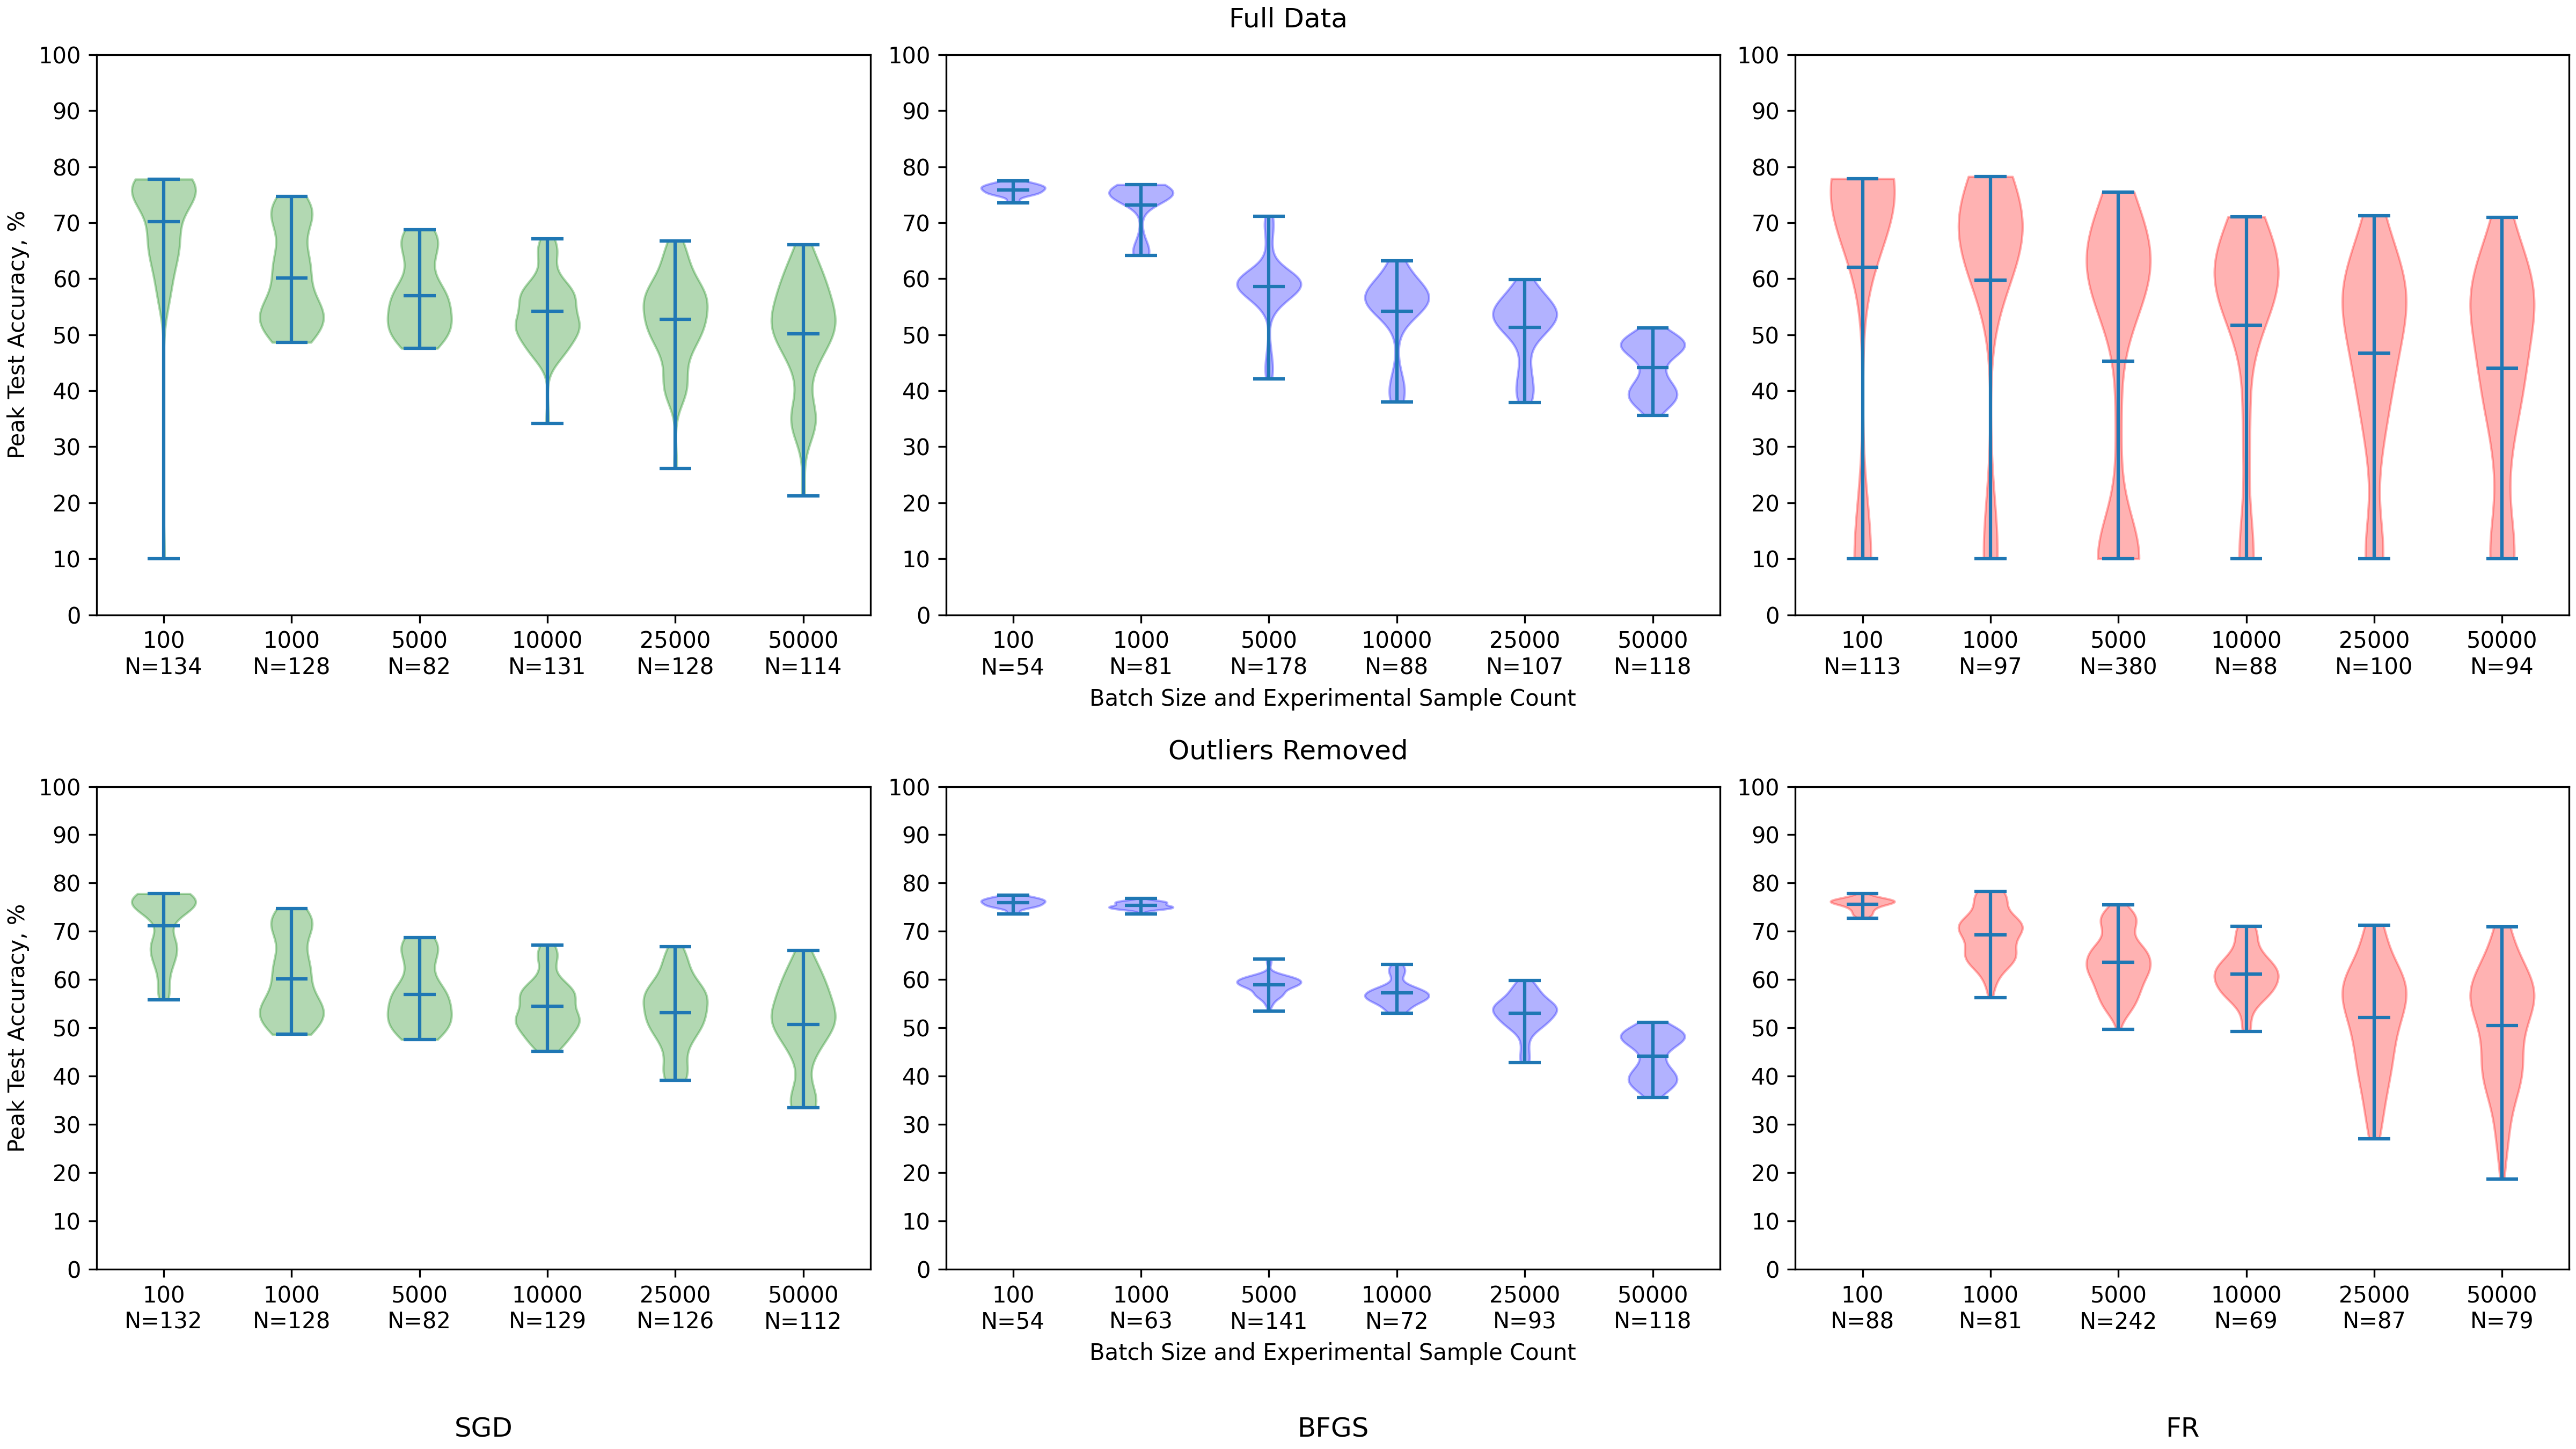
\includegraphics[width=\columnwidth]{peak_acc_violin_comparison.png}
        \end{figure}

        \begin{figure}
          \centering
          \textbf{Optimizer Time to Peak Test Accuracy in 100 Epochs (Log-linear)}
          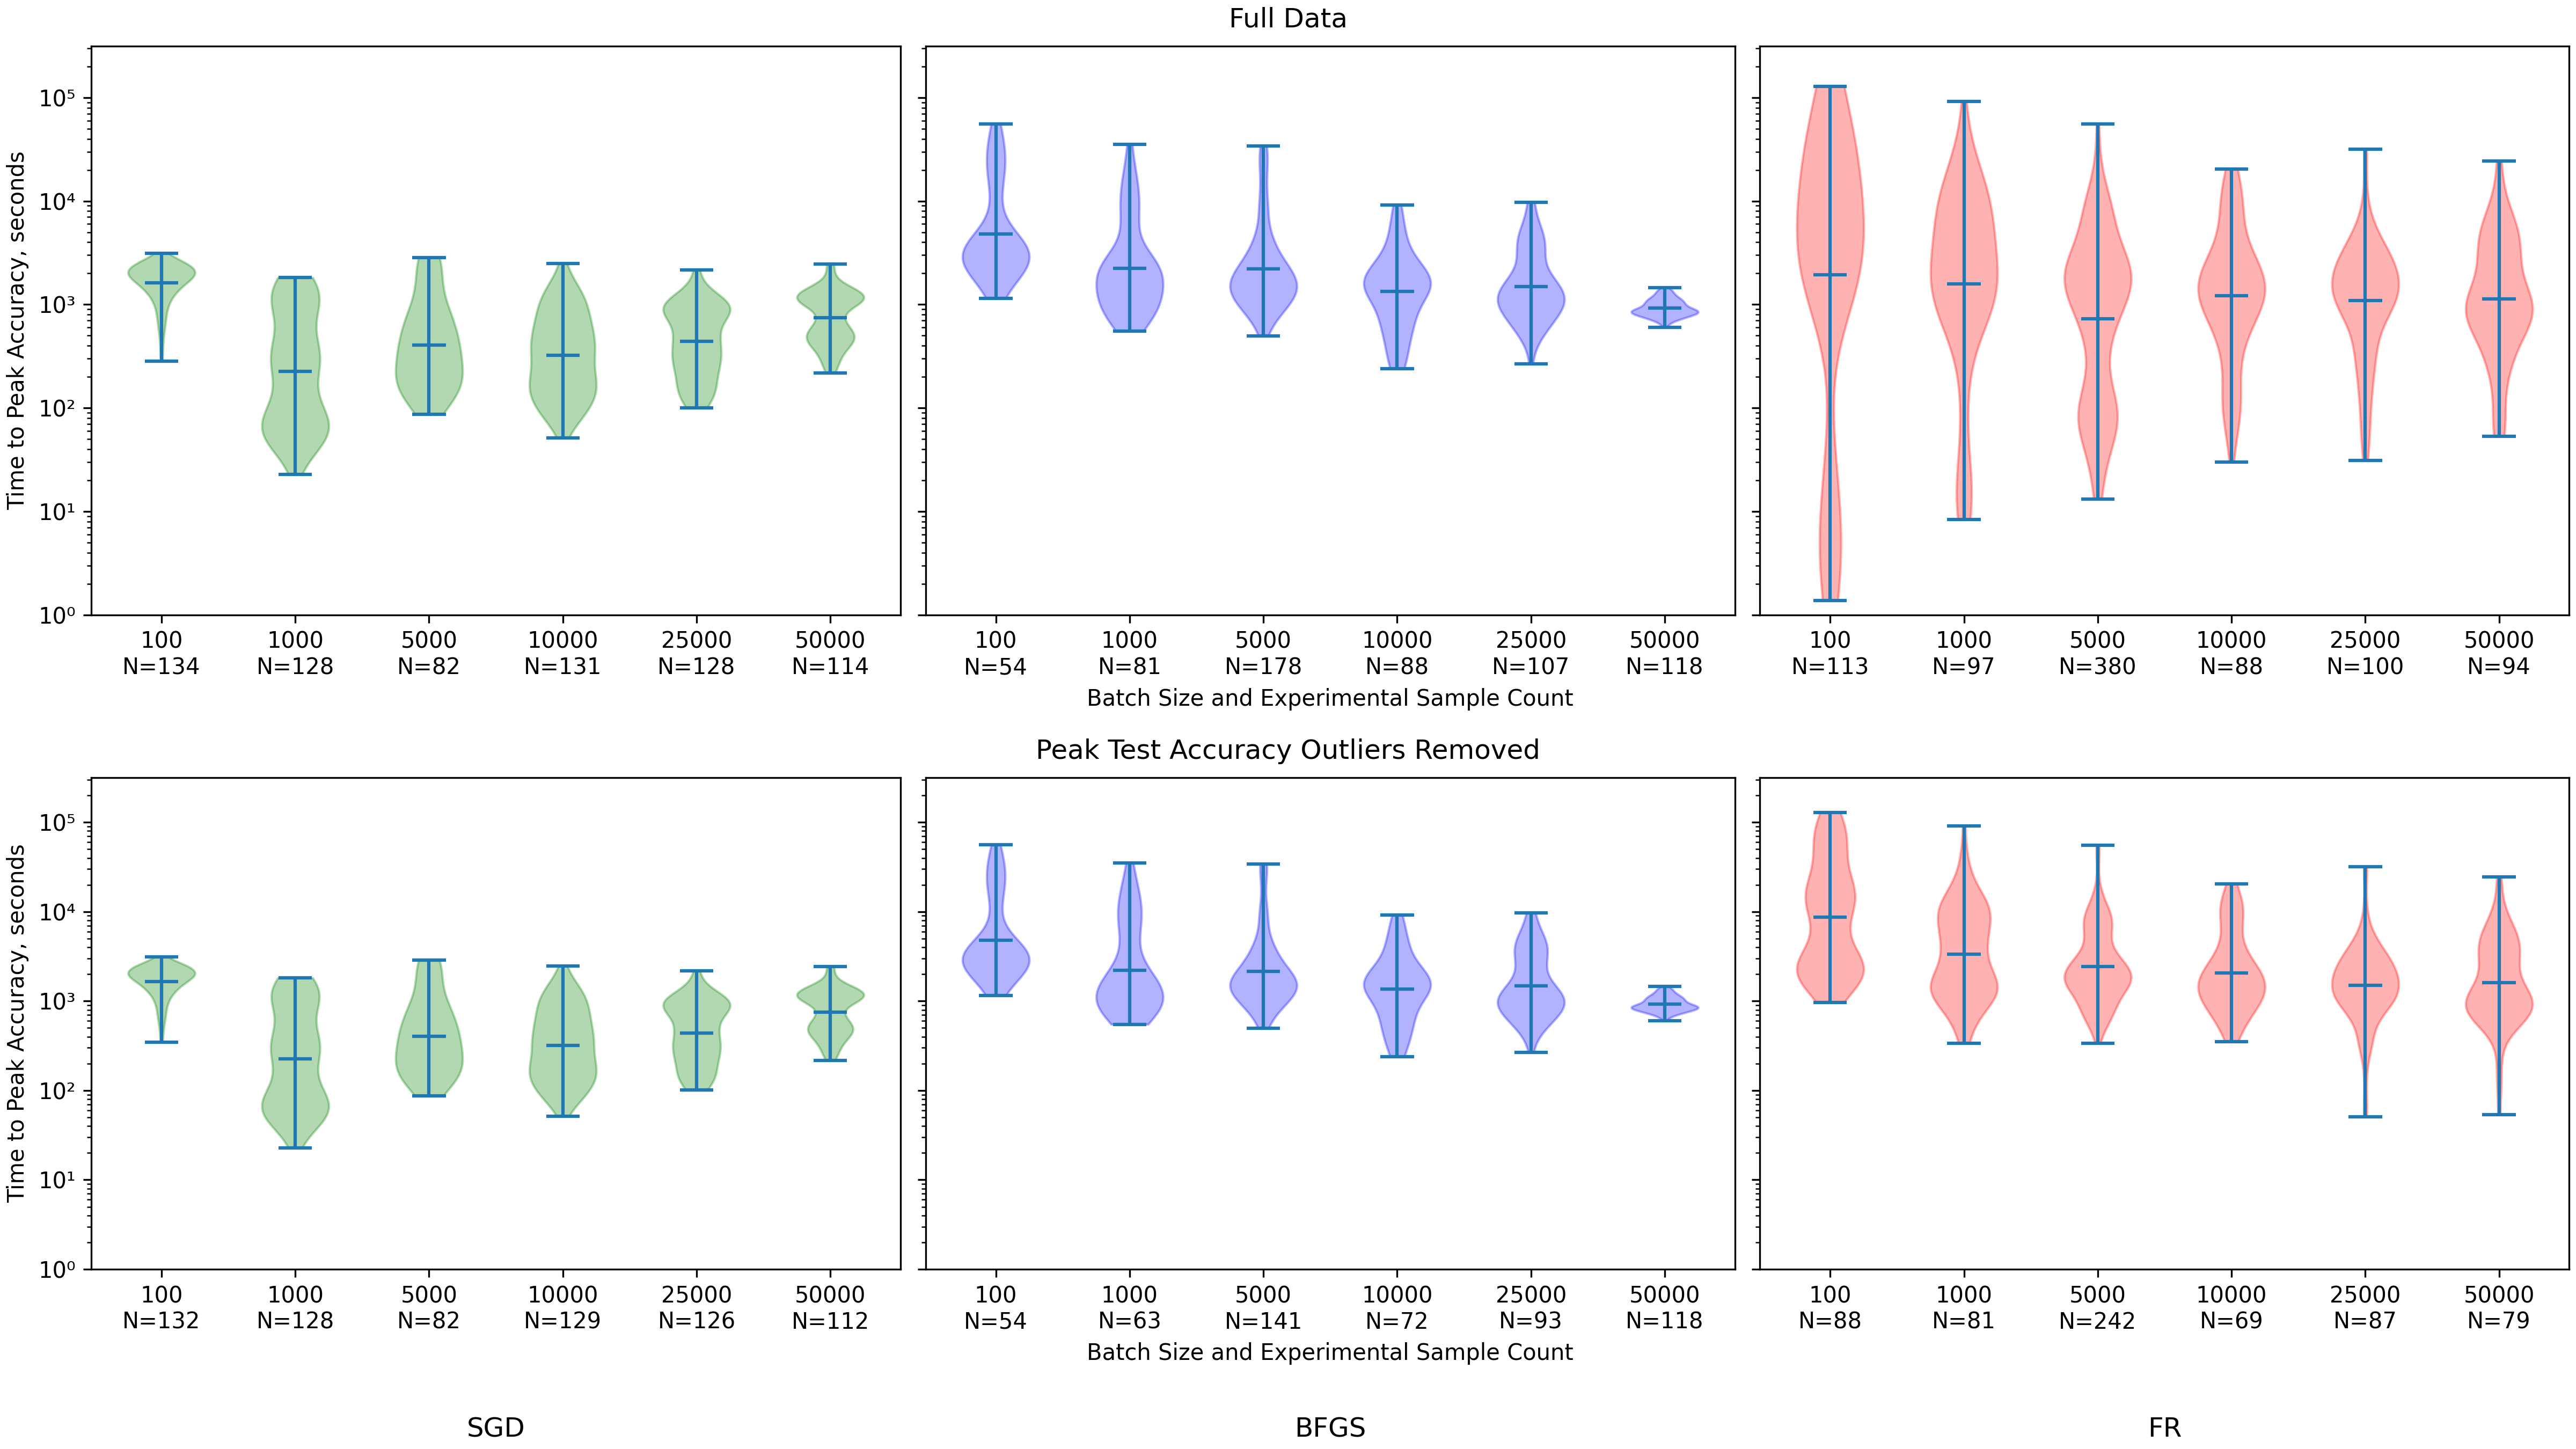
\includegraphics[width=\columnwidth]{ttp_violin_comparison.png}
        \end{figure}
        \begin{table}[]
          \begin{tabular}{|llllll|}
            \hline
            \multicolumn{6}{|c|}{\textbf{ANOVA Table with Outlier Treatment}}                                                                                                      \\ \hline
            \multicolumn{1}{|l|}{Source} & \multicolumn{1}{l|}{DF} & \multicolumn{1}{l|}{Type III SS} & \multicolumn{1}{l|}{Mean Square} & \multicolumn{1}{l|}{F Value} & PR$>$F   \\ \hline
            Batch Size                   & 5                       & 35.92                            & 7.18                             & 480.66                       & $<0.001$ \\
            Optimizer                    & 2                       & 1.37                             & 0.684                            & 45.78                        & $<0.001$ \\
            Interaction                  & 10                      & 4.11                             & 0.41                             & 27.51                        & $<0.001$ \\ \hline
          \end{tabular}
        \end{table}


      \end{block}

    \end{column}

    \separatorcolumn

    \begin{column}{\colwidth}
      \begin{block}{Results, continued}
        \begin{table}[]
          \begin{tabular}{|llll|}
            \hline
            \multicolumn{4}{|c|}{\textbf{Pairwise Tests for Interaction Effects with Outlier Treatment}}                                             \\ \hline
            \multicolumn{1}{|l|}{Batch Size} & \multicolumn{1}{l|}{Treatment} & \multicolumn{1}{l|}{LS Means} & \multicolumn{1}{c|}{Letter Grouping} \\ \hline
            \multicolumn{1}{|l|}{100}        & \multicolumn{1}{l|}{L-BFGS}    & \multicolumn{1}{l|}{4.3292}   & \multicolumn{1}{c|}{A}               \\
            \multicolumn{1}{|l|}{100}        & \multicolumn{1}{l|}{FR}        & \multicolumn{1}{l|}{4.3256}   & \multicolumn{1}{c|}{A}               \\
            \multicolumn{1}{|l|}{100}        & \multicolumn{1}{l|}{SGD}       & \multicolumn{1}{l|}{4.2597}   & \multicolumn{1}{c|}{A}               \\ \hline
            \multicolumn{1}{|l|}{1000}       & \multicolumn{1}{l|}{L-BFGS}    & \multicolumn{1}{l|}{4.3222}   & \multicolumn{1}{c|}{A}               \\
            \multicolumn{1}{|l|}{1000}       & \multicolumn{1}{l|}{FR}        & \multicolumn{1}{l|}{4.2354}   & \multicolumn{1}{c|}{B}               \\
            \multicolumn{1}{|l|}{1000}       & \multicolumn{1}{l|}{SGD}       & \multicolumn{1}{l|}{4.0879}   & \multicolumn{1}{c|}{C}               \\ \hline
            \multicolumn{1}{|l|}{5000}       & \multicolumn{1}{l|}{FR}        & \multicolumn{1}{l|}{4.1471}   & \multicolumn{1}{c|}{A}               \\
            \multicolumn{1}{|l|}{5000}       & \multicolumn{1}{l|}{L-BFGS}    & \multicolumn{1}{l|}{4.0456}   & \multicolumn{1}{c|}{B}               \\
            \multicolumn{1}{|l|}{5000}       & \multicolumn{1}{l|}{SGD}       & \multicolumn{1}{l|}{4.0358}   & \multicolumn{1}{c|}{B}               \\ \hline
            \multicolumn{1}{|l|}{10000}      & \multicolumn{1}{l|}{FR}        & \multicolumn{1}{l|}{4.2354}   & \multicolumn{1}{c|}{A}               \\
            \multicolumn{1}{|l|}{10000}      & \multicolumn{1}{l|}{L-BFGS}    & \multicolumn{1}{l|}{4.0456}   & \multicolumn{1}{c|}{A}               \\
            \multicolumn{1}{|l|}{10000}      & \multicolumn{1}{l|}{SGD}       & \multicolumn{1}{l|}{3.9925}   & \multicolumn{1}{c|}{B}               \\ \hline
            \multicolumn{1}{|l|}{25000}      & \multicolumn{1}{l|}{L-BFGS}    & \multicolumn{1}{l|}{3.9687}   & \multicolumn{1}{c|}{A}               \\
            \multicolumn{1}{|l|}{25000}      & \multicolumn{1}{l|}{SGD}       & \multicolumn{1}{l|}{3.9644}   & \multicolumn{1}{c|}{A}               \\
            \multicolumn{1}{|l|}{25000}      & \multicolumn{1}{l|}{FR}        & \multicolumn{1}{l|}{3.9288}   & \multicolumn{1}{c|}{A}               \\ \hline
            \multicolumn{1}{|l|}{50000}      & \multicolumn{1}{l|}{SGD}       & \multicolumn{1}{l|}{3.9089}   & \multicolumn{1}{c|}{A}               \\
            \multicolumn{1}{|l|}{50000}      & \multicolumn{1}{l|}{FR}        & \multicolumn{1}{l|}{3.8894}   & \multicolumn{1}{c|}{A}               \\
            \multicolumn{1}{|l|}{50000}      & \multicolumn{1}{l|}{L-BFGS}    & \multicolumn{1}{l|}{3.782}    & \multicolumn{1}{c|}{B}               \\ \hline
          \end{tabular}
        \end{table}
      \end{block}

      \begin{exampleblock}{Open Source Implementation}
        All source code is available at: \href{https://github.com/pnnl/pytorch_soo}{github.com/pnnl/pytorch\_soo}\newline
        Please feel free to use, cite, and open PR's!

      \end{exampleblock}


      \begin{block}{Conclusion}
        We have provided \textbf{strong, empirical} evidence for the often
        discussed effect of ``implicit regularization'' afforded by
        minibatching: decreased batch size produces increased peak accuracy.
        This effect \textbf{generalizes across optimizers}. This implies that
        acceleration via increased hardware utilization through larger batch
        sizes is likely not a viable research direction under the current
        paradigm. SOOs demonstrate \textbf{improved convergence results in peak
          accuracy}, both through \textbf{higher mean and lower variance}.
        Considering batch size as a a hyperparameter, this strongly indicates
        \textbf{not all hyperparameters are equally important}.  While they
        exhibit slower wall-clock performance, this insensitivity to other
        hyperparameters suggests that \textbf{hyperoptimization efforts may not
          be needed}, providing \textbf{amortized time savings}. This reduces cost,
        complexity, and increases confidence in the results of a training
        session.
      \end{block}

      \begin{block}{Aknowledgements}
        The authors wish to thank PNNL for providing the funding and compute resources to make this scale
        of a study possible.

        A special thanks to Dr. Tony Chiang, Dr. Andrew Lumsdaine, and Dr. Nairanjana Dasgupta for
        their unrelenting support on this project.
      \end{block}

    \end{column}

    \separatorcolumn
  \end{columns}
\end{frame}

\end{document}
